%%%%%%%%%%%%%%%%%%%%%%%%%%%%%%%%%%%%%%%%%%%%%%%%%%%%%%%%%%%%%%%
%% OXFORD THESIS TEMPLATE

% Use this template to produce a standard thesis that meets the Oxford University requirements for DPhil submission
%
% Originally by Keith A. Gillow (gillow@maths.ox.ac.uk), 1997
% Modified by Sam Evans (sam@samuelevansresearch.org), 2007
% Modified by John McManigle (john@oxfordechoes.com), 2015
% Modified by Ulrik Lyngs (ulrik.lyngs@cs.ox.ac.uk), 2018, for use with R Markdown
%
% Ulrik Lyngs, 25 Nov 2018: Following John McManigle, broad permissions are granted to use, modify, and distribute this software
% as specified in the MIT License included in this distribution's LICENSE file.
%
% John tried to comment this file extensively, so read through it to see how to use the various options.  Remember
% that in LaTeX, any line starting with a % is NOT executed.  Several places below, you have a choice of which line to use
% out of multiple options (eg draft vs final, for PDF vs for binding, etc.)  When you pick one, add a % to the beginning of
% the lines you don't want.


%%%%% CHOOSE PAGE LAYOUT
% The most common choices should be below.  You can also do other things, like replacing "a4paper" with "letterpaper", etc.

% This one will format for two-sided binding (ie left and right pages have mirror margins; blank pages inserted where needed):
%\documentclass[a4paper,twoside]{templates/ociamthesis}
% This one will format for one-sided binding (ie left margin > right margin; no extra blank pages):
%\documentclass[a4paper]{ociamthesis}
% This one will format for PDF output (ie equal margins, no extra blank pages):
%\documentclass[a4paper,nobind]{templates/ociamthesis}
%UL 2 Dec 2018: pass this in from YAML
\documentclass[a4paper, twoside]{templates/ociamthesis}


% UL 30 Nov 2018 pandoc puts lists in 'tightlist' command when no space between bullet points in Rmd file
\providecommand{\tightlist}{%
  \setlength{\itemsep}{0pt}\setlength{\parskip}{0pt}}
 
% UL 1 Dec 2018, fix to include code in shaded environments
\usepackage{color}
\usepackage{fancyvrb}
\newcommand{\VerbBar}{|}
\newcommand{\VERB}{\Verb[commandchars=\\\{\}]}
\DefineVerbatimEnvironment{Highlighting}{Verbatim}{commandchars=\\\{\}}
% Add ',fontsize=\small' for more characters per line
\usepackage{framed}
\definecolor{shadecolor}{RGB}{248,248,248}
\newenvironment{Shaded}{\begin{snugshade}}{\end{snugshade}}
\newcommand{\AlertTok}[1]{\textcolor[rgb]{0.94,0.16,0.16}{#1}}
\newcommand{\AnnotationTok}[1]{\textcolor[rgb]{0.56,0.35,0.01}{\textbf{\textit{#1}}}}
\newcommand{\AttributeTok}[1]{\textcolor[rgb]{0.77,0.63,0.00}{#1}}
\newcommand{\BaseNTok}[1]{\textcolor[rgb]{0.00,0.00,0.81}{#1}}
\newcommand{\BuiltInTok}[1]{#1}
\newcommand{\CharTok}[1]{\textcolor[rgb]{0.31,0.60,0.02}{#1}}
\newcommand{\CommentTok}[1]{\textcolor[rgb]{0.56,0.35,0.01}{\textit{#1}}}
\newcommand{\CommentVarTok}[1]{\textcolor[rgb]{0.56,0.35,0.01}{\textbf{\textit{#1}}}}
\newcommand{\ConstantTok}[1]{\textcolor[rgb]{0.00,0.00,0.00}{#1}}
\newcommand{\ControlFlowTok}[1]{\textcolor[rgb]{0.13,0.29,0.53}{\textbf{#1}}}
\newcommand{\DataTypeTok}[1]{\textcolor[rgb]{0.13,0.29,0.53}{#1}}
\newcommand{\DecValTok}[1]{\textcolor[rgb]{0.00,0.00,0.81}{#1}}
\newcommand{\DocumentationTok}[1]{\textcolor[rgb]{0.56,0.35,0.01}{\textbf{\textit{#1}}}}
\newcommand{\ErrorTok}[1]{\textcolor[rgb]{0.64,0.00,0.00}{\textbf{#1}}}
\newcommand{\ExtensionTok}[1]{#1}
\newcommand{\FloatTok}[1]{\textcolor[rgb]{0.00,0.00,0.81}{#1}}
\newcommand{\FunctionTok}[1]{\textcolor[rgb]{0.00,0.00,0.00}{#1}}
\newcommand{\ImportTok}[1]{#1}
\newcommand{\InformationTok}[1]{\textcolor[rgb]{0.56,0.35,0.01}{\textbf{\textit{#1}}}}
\newcommand{\KeywordTok}[1]{\textcolor[rgb]{0.13,0.29,0.53}{\textbf{#1}}}
\newcommand{\NormalTok}[1]{#1}
\newcommand{\OperatorTok}[1]{\textcolor[rgb]{0.81,0.36,0.00}{\textbf{#1}}}
\newcommand{\OtherTok}[1]{\textcolor[rgb]{0.56,0.35,0.01}{#1}}
\newcommand{\PreprocessorTok}[1]{\textcolor[rgb]{0.56,0.35,0.01}{\textit{#1}}}
\newcommand{\RegionMarkerTok}[1]{#1}
\newcommand{\SpecialCharTok}[1]{\textcolor[rgb]{0.00,0.00,0.00}{#1}}
\newcommand{\SpecialStringTok}[1]{\textcolor[rgb]{0.31,0.60,0.02}{#1}}
\newcommand{\StringTok}[1]{\textcolor[rgb]{0.31,0.60,0.02}{#1}}
\newcommand{\VariableTok}[1]{\textcolor[rgb]{0.00,0.00,0.00}{#1}}
\newcommand{\VerbatimStringTok}[1]{\textcolor[rgb]{0.31,0.60,0.02}{#1}}
\newcommand{\WarningTok}[1]{\textcolor[rgb]{0.56,0.35,0.01}{\textbf{\textit{#1}}}}
%UL 2 Dec 2018 add a bit of white space before and after code blocks
\renewenvironment{Shaded}
{
  \vspace{4pt}%
  \begin{snugshade}%
}{%
  \end{snugshade}%
  \vspace{4pt}%
}

%UL 2 Dec 2018 reduce whitespace around verbatim environments
\usepackage{etoolbox}
\makeatletter
\preto{\@verbatim}{\topsep=0pt \partopsep=0pt }
\makeatother

%UL 26 Mar 2019, enable strikethrough
\usepackage[normalem]{ulem}

%UL 15 Oct 2019, enable link highlighting to be turned off from YAML
\usepackage[colorlinks=false,pdfpagelabels,hidelinks=true]{hyperref}

%%%%% SELECT YOUR DRAFT OPTIONS
% Three options going on here; use in any combination.  But remember to turn the first two off before
% generating a PDF to send to the printer!

% This adds a "DRAFT" footer to every normal page.  (The first page of each chapter is not a "normal" page.)
\fancyfoot[C]{\emph{DRAFT Printed on \today}}

% This highlights (in blue) corrections marked with (for words) \mccorrect{blah} or (for whole
% paragraphs) \begin{mccorrection} . . . \end{mccorrection}.  This can be useful for sending a PDF of
% your corrected thesis to your examiners for review.  Turn it off, and the blue disappears.
\correctionstrue

%%%%% BIBLIOGRAPHY SETUP
% Note that your bibliography will require some tweaking depending on your department, preferred format, etc.
% The options included below are just very basic "sciencey" and "humanitiesey" options to get started.
% If you've not used LaTeX before, I recommend reading a little about biblatex/biber and getting started with it.
% If you're already a LaTeX pro and are used to natbib or something, modify as necessary.
% Either way, you'll have to choose and configure an appropriate bibliography format...

% The science-type option: numerical in-text citation with references in order of appearance.
% \usepackage[style=numeric-comp, sorting=none, backend=biber, doi=false, isbn=false]{biblatex}
% \newcommand*{\bibtitle}{References}

% The humanities-type option: author-year in-text citation with an alphabetical works cited.
% \usepackage[style=authoryear, sorting=nyt, backend=biber, maxcitenames=2, useprefix, doi=false, isbn=false]{biblatex}
% \newcommand*{\bibtitle}{Works Cited}

%UL 3 Dec 2018: set this from YAML in index.Rmd
\usepackage[style=apa, sorting=nyt, backend=biber, maxcitenames=2, useprefix, doi=true, isbn=false, uniquename=false]{biblatex}
\newcommand*{\bibtitle}{Works Cited}


% This makes the bibliography left-aligned (not 'justified') and slightly smaller font.
\renewcommand*{\bibfont}{\raggedright\small}

% Change this to the name of your .bib file (usually exported from a citation manager like Zotero or EndNote).
\addbibresource{references.bib}


% Uncomment this if you want equation numbers per section (2.3.12), instead of per chapter (2.18):
%\numberwithin{equation}{subsection}


%%%%% THESIS / TITLE PAGE INFORMATION
% Everybody needs to complete the following:
\title{My thesis title\\
Title second row}
\author{Shiran Koifman}
\college{}

% Master's candidates who require the alternate title page (with candidate number and word count)
% must also un-comment and complete the following three lines:
%\masterssubmissiontrue
%\candidateno{933516}
%\wordcount{28,815}

% Uncomment the following line if your degree also includes exams (eg most masters):
%\renewcommand{\submittedtext}{Submitted in partial completion of the}
% Your full degree name.  (But remember that DPhils aren't "in" anything.  They're just DPhils.)
\degree{}
% Term and year of submission, or date if your board requires (eg most masters)
\degreedate{January 15 2021}


%%%%% YOUR OWN PERSONAL MACROS
% This is a good place to dump your own LaTeX macros as they come up.

% To make text superscripts shortcuts
	\renewcommand{\th}{\textsuperscript{th}} % ex: I won 4\th place
	\newcommand{\nd}{\textsuperscript{nd}}
	\renewcommand{\st}{\textsuperscript{st}}
	\newcommand{\rd}{\textsuperscript{rd}}

%%%%% THE ACTUAL DOCUMENT STARTS HERE
\begin{document}

%%%%% CHOOSE YOUR LINE SPACING HERE
% This is the official option.  Use it for your submission copy and library copy:
\setlength{\textbaselineskip}{22pt plus2pt}
% This is closer spacing (about 1.5-spaced) that you might prefer for your personal copies:
%\setlength{\textbaselineskip}{18pt plus2pt minus1pt}

% You can set the spacing here for the roman-numbered pages (acknowledgements, table of contents, etc.)
\setlength{\frontmatterbaselineskip}{17pt plus1pt minus1pt}

% UL: You can set the line and paragraph spacing here for the separate abstract page to be handed in to Examination schools
\setlength{\abstractseparatelineskip}{13pt plus1pt minus1pt}
\setlength{\abstractseparateparskip}{0pt plus 1pt}

% UL: You can set the general paragraph spacing here - I've set it to 2pt (was 0) so
% it's less claustrophobic
\setlength{\parskip}{2pt plus 1pt}


% Leave this line alone; it gets things started for the real document.
\setlength{\baselineskip}{\textbaselineskip}


%%%%% CHOOSE YOUR SECTION NUMBERING DEPTH HERE
% You have two choices.  First, how far down are sections numbered?  (Below that, they're named but
% don't get numbers.)  Second, what level of section appears in the table of contents?  These don't have
% to match: you can have numbered sections that don't show up in the ToC, or unnumbered sections that
% do.  Throughout, 0 = chapter; 1 = section; 2 = subsection; 3 = subsubsection, 4 = paragraph...

% The level that gets a number:
\setcounter{secnumdepth}{2}
% The level that shows up in the ToC:
\setcounter{tocdepth}{2}


%%%%% ABSTRACT SEPARATE
% This is used to create the separate, one-page abstract that you are required to hand into the Exam
% Schools.  You can comment it out to generate a PDF for printing or whatnot.

% JEM: Pages are roman numbered from here, though page numbers are invisible until ToC.  This is in
% keeping with most typesetting conventions.
\begin{romanpages}

% Title page is created here
\maketitle

%%%%% DEDICATION -- If you'd like one, un-comment the following.
\begin{dedication}
  For Yihui Xie
\end{dedication}

%%%%% ACKNOWLEDGEMENTS -- Nothing to do here except comment out if you don't want it.
\begin{acknowledgements}
 	This is where you will normally thank your advisor, colleagues, family and friends, as well as funding and institutional support. In our case, we will give our praises to the people who developed the ideas and tools that allow us to push open science a little step forward by writing plain-text, transparent, and reproducible theses in R Markdown.

  We must be grateful to John Gruber for inventing the original version of Markdown, to John MacFarlane for creating Pandoc (\url{http://pandoc.org}) which converts Markdown to a large number of output formats, and to Yihui Xie for creating \texttt{knitr} which introduced R Markdown as a way of embedding code in Markdown documents, and \texttt{bookdown} which added tools for technical and longer-form writing.

  Special thanks to \href{http://chester.rbind.io}{Chester Ismay}, who created the \texttt{thesisdown} package that helped many a PhD student write their theses in R Markdown. And a very special tahnks to John McManigle, whose adaption of Sam Evans' adaptation of Keith Gillow's original maths template for writing an Oxford University DPhil thesis in \LaTeX~provided the template that I adapted for R Markdown.

  Finally, profuse thanks to JJ Allaire, the founder and CEO of \href{http://rstudio.com}{RStudio}, and Hadley Wickham, the mastermind of the tidyverse without whom we'd all just given up and done data science in Python instead. Thanks for making data science easier, more accessible, and more fun for us all.

  \begin{flushright}
  Ulrik Lyngs \\
  Linacre College, Oxford \\
  2 December 2018
  \end{flushright}
\end{acknowledgements}


%%%%% ABSTRACT -- Nothing to do here except comment out if you don't want it.
\begin{abstract}
	This \emph{R Markdown} template is for writing an Oxford University thesis. The template is built using Yihui Xie's \texttt{bookdown} package, with heavy inspiration from Chester Ismay's \texttt{thesisdown} and the \texttt{OxThesis} \LaTeX~template (most recently adapted by John McManigle).

 This template's sample content include illustrations of how to write a thesis in R Markdown, and largely follows the structure from \href{https://ulyngs.github.io/rmarkdown-workshop-2019/}{this R Markdown workshop}.

 Congratulations for taking a step further into the lands of open, reproducible science by writing your thesis using a tool that allows you to transparently include tables and dynamically generated plots directly from the underlying data. Hip hooray!
\end{abstract}

%%%%% MINI TABLES
% This lays the groundwork for per-chapter, mini tables of contents.  Comment the following line
% (and remove \minitoc from the chapter files) if you don't want this.  Un-comment either of the
% next two lines if you want a per-chapter list of figures or tables.
  \dominitoc % include a mini table of contents

% This aligns the bottom of the text of each page.  It generally makes things look better.
\flushbottom

% This is where the whole-document ToC appears:
\tableofcontents

\listoffigures
	\mtcaddchapter
  	% \mtcaddchapter is needed when adding a non-chapter (but chapter-like) entity to avoid confusing minitoc

% Uncomment to generate a list of tables:
\listoftables
  \mtcaddchapter
%%%%% LIST OF ABBREVIATIONS
% This example includes a list of abbreviations.  Look at text/abbreviations.tex to see how that file is
% formatted.  The template can handle any kind of list though, so this might be a good place for a
% glossary, etc.
% First parameter can be changed eg to "Glossary" or something.
% Second parameter is the max length of bold terms.
\begin{mclistof}{List of Abbreviations}{3.2cm}

\item[1-D, 2-D] One- or two-dimensional, referring in this thesis to spatial dimensions in an image.

\item[Otter] One of the finest of water mammals.

\item[Hedgehog] Quite a nice prickly friend.

\end{mclistof} 


% The Roman pages, like the Roman Empire, must come to its inevitable close.
\end{romanpages}

%%%%% CHAPTERS
% Add or remove any chapters you'd like here, by file name (excluding '.tex'):
\flushbottom

% all your chapters and appendices will appear here
\hypertarget{introduction}{%
\chapter*{Introduction}\label{introduction}}
\addcontentsline{toc}{chapter}{Introduction}

\adjustmtc

Welcome to the \emph{R Markdown} Oxford University thesis template.
This sample content is adapted from \href{https://github.com/ismayc/thesisdown}{\texttt{thesisdown}} and the formatting of PDF output is adapted from the \href{https://github.com/mcmanigle/OxThesis}{OxThesis LaTeX template}.
Hopefully, writing your thesis in R Markdown will provide a nicer interface to the OxThesis template if you haven't used TeX or LaTeX before.
More importantly, using \emph{R Markdown} allows you to embed chunks of code directly into your thesis and generate plots and tables directly from the underlying data, avoiding copy-paste steps.
This will get you into the habit of doing reproducible research, which benefits you long-term as a researcher, but also will greatly help anyone that is trying to reproduce or build upon your results down the road.

Using LaTeX together with \emph{Markdown} is more consistent than the output of a word processor, much less prone to corruption or crashing, and the resulting file is smaller than a Word file.
While you may never have had problems using Word in the past, your thesis is likely going to be about twice as large and complex as anything you've written before, taxing Word's capabilities.

\hypertarget{speech-in-noise-in-children}{%
\section*{Speech-in-noise in children}\label{speech-in-noise-in-children}}
\addcontentsline{toc}{section}{Speech-in-noise in children}

\emph{R Markdown} creates a simple and straightforward way to interface with the beauty of LaTeX.
Packages have been written in \textbf{R} to work directly with LaTeX to produce nicely formatting tables and paragraphs.
In addition to creating a user friendly interface to LaTeX, \emph{R Markdown} allows you to read in your data, analyze it and to visualize it using \textbf{R}, \textbf{Python} or other languages, and provide documentation and commentary on the results of your project.\\
Further, it allows for results of code output to be passed inline to the commentary of your results.
You'll see more on this later, focusing on \textbf{R}. If you are more into \textbf{Python} or something else, you can still use \emph{R Markdown} - see \href{https://bookdown.org/yihui/rmarkdown/language-engines.html}{`Other language engines'} in Yihui Xie's \href{https://bookdown.org/yihui/rmarkdown/language-engines.html}{\emph{R Markdown: The Definitive Guide}}.

\hypertarget{apd-definition}{%
\section*{APD definition}\label{apd-definition}}
\addcontentsline{toc}{section}{APD definition}

Anyone who needs to use data analysis, math, tables, a lot of figures, complex cross-references, or who just cares about reproducibility in research can benefit from using \emph{R Markdown}.
If you are working in `softer' fields, the user-friendly nature of the \emph{Markdown} syntax and its ability to keep track of and easily include figures, automatically generate a table of contents, index, references, table of figures, etc. should still make it of great benefit to your thesis project.

\hypertarget{diagnosis}{%
\section*{Diagnosis}\label{diagnosis}}
\addcontentsline{toc}{section}{Diagnosis}

Anyone who needs to use data analysis, math, tables, a lot of figures, complex cross-references, or who just cares about reproducibility in research can benefit from using \emph{R Markdown}.
If you are working in `softer' fields, the user-friendly nature of the \emph{Markdown} syntax and its ability to keep track of and easily include figures, automatically generate a table of contents, index, references, table of figures, etc. should still make it of great benefit to your thesis project.

\hypertarget{binaural-and-spatial-listening-in-apd}{%
\section*{Binaural and spatial listening in APD}\label{binaural-and-spatial-listening-in-apd}}
\addcontentsline{toc}{section}{Binaural and spatial listening in APD}

Anyone who needs to use data analysis, math, tables, a lot of figures, complex cross-references, or who just cares about reproducibility in research can benefit from using \emph{R Markdown}.
If you are working in `softer' fields, the user-friendly nature of the \emph{Markdown} syntax and its ability to keep track of and easily include figures, automatically generate a table of contents, index, references, table of figures, etc. should still make it of great benefit to your thesis project.

\hypertarget{summary}{%
\section*{Summary}\label{summary}}
\addcontentsline{toc}{section}{Summary}

Anyone who needs to use data analysis, math, tables, a lot of figures, complex cross-references, or who just cares about reproducibility in research can benefit from using \emph{R Markdown}.
If you are working in `softer' fields, the user-friendly nature of the \emph{Markdown} syntax and its ability to keep track of and easily include figures, automatically generate a table of contents, index, references, table of figures, etc. should still make it of great benefit to your thesis project.

\begin{savequote}
Neque porro quisquam est qui dolorem ipsum quia dolor sit amet,
consectetur, adipisci velit\ldots{}

There is no one who loves pain itself, who seeks after it and wants to
have it, simply because it is pain\ldots{}
\qauthor{--- Cicero's \emph{de Finibus Bonorum et Malorum}.}\end{savequote}



\hypertarget{rmd-basics}{%
\chapter{Binaural listening: interripted and alternated speech-in-noise in adults}\label{rmd-basics}}

\minitoc 

Here is a brief introduction to using \emph{R Markdown}.
\emph{Markdown} is a simple formatting syntax for authoring HTML, PDF, and MS Word documents and much, much more.
\emph{R Markdown} provides the flexibility of \emph{Markdown} with the implementation of \textbf{R} input and output. For more details on using \emph{R Markdown} see \url{http://rmarkdown.rstudio.com}.

Be careful with your spacing in \emph{Markdown} documents.
While whitespace largely is ignored, it does at times give \emph{Markdown} signals as to how to proceed.
As a habit, try to keep everything left aligned whenever possible, especially as you type a new paragraph.
In other words, there is no need to indent basic text in the Rmd document (in fact, it might cause your text to do funny things if you do).

\hypertarget{influence-of-distractor-type-on-im}{%
\section{Influence of distractor type on IM}\label{influence-of-distractor-type-on-im}}

\hypertarget{introduction-1}{%
\subsection{Introduction}\label{introduction-1}}

\begin{itemize}
\tightlist
\item
  \emph{Italics} are done like *this* or \_this\_
\item
  \textbf{Bold} is done like **this** or \_\_this\_\_
\item
  \textbf{\emph{Bold and italics}} is done like ***this***, \_\_\_this\_\_\_, or (the most transparent solution, in my opinion) **\_this\_**
\end{itemize}

\hypertarget{experiment-i-speech-vs.-non-speech-distractors}{%
\subsection{Experiment I: speech vs.~non-speech distractors}\label{experiment-i-speech-vs.-non-speech-distractors}}

\begin{itemize}
\tightlist
\item
  \texttt{Inline\ code} is created with backticks like \texttt{\textasciigrave{}this\textasciigrave{}}
\end{itemize}

\hypertarget{methods}{%
\subsubsection{Methods}\label{methods}}

Sub\textsubscript{2} and super\textsuperscript{2} script is created like this\textasciitilde2\textasciitilde{} and this\^{}2\^{}

\hypertarget{results}{%
\subsubsection{Results}\label{results}}

\begin{itemize}
\tightlist
\item
  \sout{Strikethrough} is done \textasciitilde\textasciitilde like this\textasciitilde\textasciitilde{}
\end{itemize}

\hypertarget{discussion}{%
\subsubsection{Discussion}\label{discussion}}

\begin{itemize}
\tightlist
\item
  To include an actual *, \_ or \textbackslash, add another \textbackslash{} in front of them: \textbackslash*, \textbackslash\_, \textbackslash\textbackslash{}
\end{itemize}

\hypertarget{experiment-ii-speech-distractors-spoken-in-a-familiar-vs.-unfamiliar-language}{%
\subsection{Experiment II: speech distractors spoken in a familiar vs.~unfamiliar language}\label{experiment-ii-speech-distractors-spoken-in-a-familiar-vs.-unfamiliar-language}}

\begin{itemize}
\tightlist
\item
  -- and --- with -\/- and -\/-\/-
\end{itemize}

\hypertarget{methods-1}{%
\subsubsection{Methods}\label{methods-1}}

Do like this:

\begin{quote}
Put a \textgreater{} in front of the line.
\end{quote}

\hypertarget{results-1}{%
\subsubsection{Results}\label{results-1}}

\begin{itemize}
\tightlist
\item
  are done with \#'s of increasing number, i.e.~

  \begin{itemize}
  \tightlist
  \item
    \# First-level heading
  \item
    \#\# Second-level heading
  \item
    \#\#\# Etc.
  \end{itemize}
\end{itemize}

In PDF output, a level-five heading will turn into a paragraph heading, i.e.~\texttt{\textbackslash{}paragraph\{My\ level-five\ heading\}}, which appears as bold text on the same line as the subsequent paragraph.

\hypertarget{discussion-1}{%
\subsubsection{Discussion}\label{discussion-1}}

Unordered list by starting a line with an * or a -:

\begin{itemize}
\tightlist
\item
  Item 1
\item
  Item 2
\end{itemize}

Ordered lists by starting a line with a number:

\begin{enumerate}
\def\labelenumi{\arabic{enumi}.}
\tightlist
\item
  Item 1
\item
  Item 2
\end{enumerate}

Notice that you can mislabel the numbers and \emph{Markdown} will still make the order right in the output.

To create a sublist, indent the values a bit (at least four spaces or a tab):

\begin{enumerate}
\def\labelenumi{\arabic{enumi}.}
\tightlist
\item
  Item 1
\item
  Item 2
\item
  Item 3

  \begin{itemize}
  \tightlist
  \item
    Item 3a
  \item
    Item 3b
  \end{itemize}
\end{enumerate}

\hypertarget{general-discussion-and-conclusion}{%
\subsection{General discussion and conclusion}\label{general-discussion-and-conclusion}}

The official \emph{Markdown} way to create line breaks is by ending a line with more than two spaces.

Roses are red.
Violets are blue.

This appears on the same line in the output, because we didn't add spaces after red.

Roses are red.\\
Violets are blue.

This appears with a line break because I added spaces after red.

I find this is confusing, so I recommend the alternative way: Ending a line with a backslash will also create a linebreak:

Roses are red.\\
Violets are blue.

To create a new paragraph, you put a blank line.

Therefore, this line starts its own paragraph.

\hypertarget{dichotic-vs.-monotic-presentation-and-the-influence-of-speech-material}{%
\section{Dichotic vs.~monotic presentation and the influence of speech material}\label{dichotic-vs.-monotic-presentation-and-the-influence-of-speech-material}}

\begin{itemize}
\tightlist
\item
  \href{https://www.google.com}{This is a hyperlink} created by writing the text you want turned into a clickable link in \texttt{{[}square\ brackets\ followed\ by\ a{]}(https://hyperlink-in-parentheses)}
\end{itemize}

\hypertarget{introduction-2}{%
\subsection{Introduction}\label{introduction-2}}

\begin{itemize}
\tightlist
\item
  Are created\footnote{my footnote text} by writing either \^{}{[}my footnote text{]} for supplying the footnote content inline, or something like \texttt{{[}\^{}a-random-footnote-label{]}} and supplying the text elsewhere in the format shown below \footnote{This is a random test.}:
\end{itemize}

\texttt{{[}\^{}a-random-footnote-label{]}:\ This\ is\ a\ random\ test.}

\hypertarget{methods-2}{%
\subsection{Methods}\label{methods-2}}

To write comments within your text that won't actually be included in the output, use the same syntax as for writing comments in HTML. That is, \textless!-\/- this will not be included in the output -\/-\textgreater.

\hypertarget{results-2}{%
\subsection{Results}\label{results-2}}

The syntax for writing math is stolen from LaTeX. To write a math expression that will be shown \textbf{inline}, enclose it in dollar signs.
- This: \$A = \textbackslash pi*r\^{}\{2\}\$ Becomes: \(A = \pi*r^{2}\)

To write a math expression that will be shown in a block, enclose it in two dollar signs.\\
This: \$\$A = \textbackslash pi*r\^{}\{2\}\$\$

Becomes:
\[A = \pi*r^{2}\]

To create numbered equations, put them in an `equation' environment and give them a label with the syntax \texttt{(\textbackslash{}\#eq:label)}, like this:

\begin{Shaded}
\begin{Highlighting}[]
\KeywordTok{\textbackslash{}begin}\NormalTok{\{}\ExtensionTok{equation}\NormalTok{\}}\SpecialStringTok{ }
\SpecialStringTok{  f}\SpecialCharTok{\textbackslash{}left}\SpecialStringTok{(k}\SpecialCharTok{\textbackslash{}right}\SpecialStringTok{) = }\SpecialCharTok{\textbackslash{}binom}\SpecialStringTok{\{n\}\{k\} p\^{}k}\SpecialCharTok{\textbackslash{}left}\SpecialStringTok{(1{-}p}\SpecialCharTok{\textbackslash{}right}\SpecialStringTok{)\^{}\{n{-}k\}}
\SpecialStringTok{  (}\SpecialCharTok{\textbackslash{}\#}\SpecialStringTok{eq:binom)}
\KeywordTok{\textbackslash{}end}\NormalTok{\{}\ExtensionTok{equation}\NormalTok{\} }
\end{Highlighting}
\end{Shaded}

Becomes:
\begin{equation}
f\left(k\right)=\binom{n}{k}p^k\left(1-p\right)^{n-k}
\label{eq:binom}
\end{equation}

For more (e.g.~how to theorems), see e.g.~the documentation on \href{https://bookdown.org/yihui/bookdown/markdown-extensions-by-bookdown.html\#equations}{bookdown.org}

\hypertarget{discussion-2}{%
\subsection{Discussion}\label{discussion-2}}

\begin{itemize}
\item
  \emph{R Markdown: The Definitive Guide} - \url{https://bookdown.org/yihui/rmarkdown/}
\item
  \emph{R for Data Science} - \url{https://r4ds.had.co.nz}
\end{itemize}

\hypertarget{conclusion}{%
\subsection{Conclusion}\label{conclusion}}

\hypertarget{code}{%
\chapter{Spatial listening: development and normalisation of a children's spatialised speech-in-noise test}\label{code}}

\minitoc 

The magic of R Markdown is that we can add code within our document to make it dynamic.

We do this either as \emph{code chunks} (generally used for loading libraries and data, performing calculations, and adding images, plots, and tables), or \emph{inline code} (generally used for dynamically reporting results within our text).

\hypertarget{introduction-3}{%
\section{Introduction}\label{introduction-3}}

\hypertarget{methods-3}{%
\section{Methods}\label{methods-3}}

\hypertarget{discussion-3}{%
\section{Discussion}\label{discussion-3}}

\hypertarget{conclusion-1}{%
\section{Conclusion}\label{conclusion-1}}

The syntax of a code chunk is shown in Figure \ref{fig:chunk-parts}.

\begin{figure}
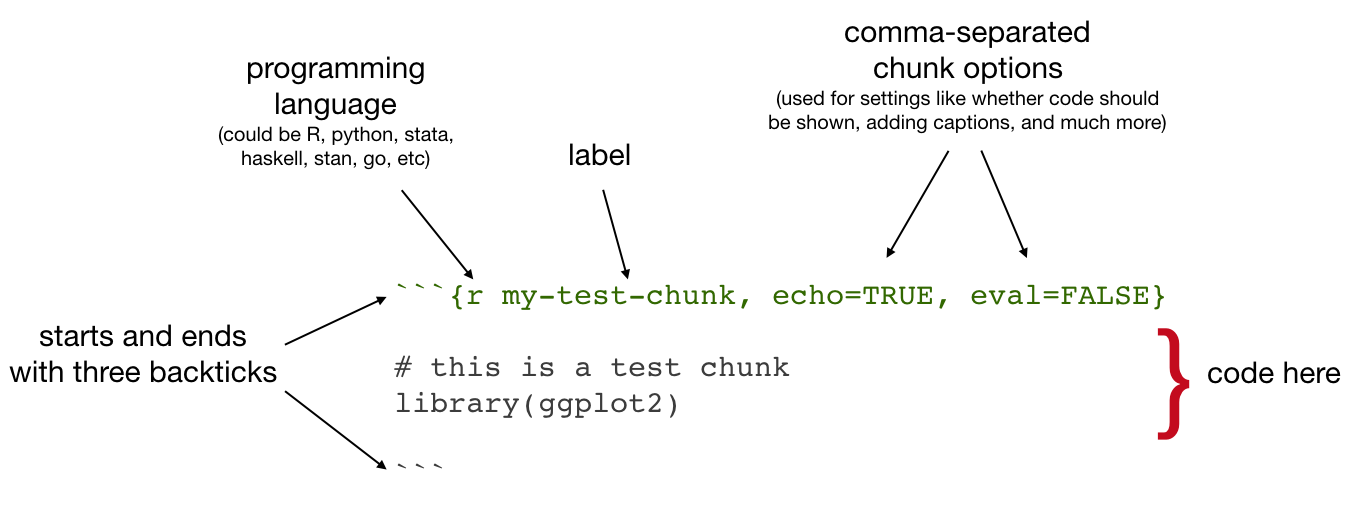
\includegraphics[width=1\linewidth]{figures/chunk-parts} \caption{Code chunk syntax}\label{fig:chunk-parts}
\end{figure}

Common chunk options include (see e.g.~\href{https://bookdown.org/yihui/rmarkdown/r-code.html}{bookdown.org}):

\begin{itemize}
\tightlist
\item
  \texttt{echo}: whether or not to display code in knitted output
\item
  \texttt{eval}: whether or to to run the code in the chunk when knitting
\item
  \texttt{include}: wheter to include anything from the from a code chunk in the output document
\item
  \texttt{fig.cap}: figure caption
\item
  \texttt{fig.scap}: short figure caption, which will be used in the `List of Figures' in the PDF front matter
\end{itemize}

\textbf{IMPORTANT}: Do \emph{not} use underscoores in your chunk labels - if you do, you are likely to get an error in PDF output saying something like ``! Package caption Error: \textbackslash caption outside float''.

\hypertarget{APD-study}{%
\chapter{APD study}\label{APD-study}}

\chaptermark{APD study}

\minitoc 

\hypertarget{introduction-4}{%
\section{Introduction}\label{introduction-4}}

\hypertarget{methods-4}{%
\section{Methods}\label{methods-4}}

\hypertarget{participants}{%
\subsection{Participants}\label{participants}}

Forty-four primary school children native British English speakers with normal hearing acuity participated in the study. Amongst them 20 belonged to the APD clinical group (5 females) with an average age of 11.04 \(\pm\)~1.42 years (range: 7.8 - 12.9 years). One APD child was excluded from the analysis due to raised thresholds (PTA\textgreater25~dB~HL). APD children were recruited in two ways. Children diagnosed with APD at Great Ormond Street Hospital (GOSH) and at the London Hearing and Balance Centre (LHBC), London, UK, and fulfilled the recruitment criteria were identified and contacted by a clinical team member. The parents/caregivers were provided with information about the study and means of contact to express interest in participation. Others were recruited by advertisements in social networks, where parents were requested to fill-out an interest form that included screening questions to ensure they fulfil the participation requirements. \colorbox[HTML]{CCCCFF}{To add percentage for clinics, diagnosed/LiD/susAPD and SPD pattern?} The remaining 23 (12 females) comprised of typically developing control children (TD) with no reported concerns or diagnosis of a language or other cognitive developmental disorders. The TD group average age was 9.47 \(\pm\)~1.58 years and ranged between 7 to 12.1 years (A detailed description of the groups is shown in Tab. ??).

Difference in variance for age between the two groups was tested using t-test with Welch degrees of freedom correction for uneven sample-size, showing a significant difference in age between the groups {[}t(40.95)=3.43, p=0.001{]}.

The project was approved by the UCL Research Ethics Committee (Project ID Number 0544/006) and the NHS Health Research Authority HRA (REC reference: 18/LO/0250). The testing commenced once an informed consent was given by both the parent/caregiver and the child.

\begin{itemize}
\tightlist
\item
  Background questionnaire
\item
  Otoscopic examination was carried out to ensure the eardrum is visible, healthy and intact.
\item
  Location of the testing
\item
  duration of the session
\end{itemize}

Participants from both TD and APD group completed the same battery of tests listed below

\hypertarget{auditory-evaluation}{%
\subsection{Auditory evaluation}\label{auditory-evaluation}}

\hypertarget{standard-audiometry}{%
\subsubsection{\texorpdfstring{\textbf{Standard audiometry}}{Standard audiometry}}\label{standard-audiometry}}

\begin{figure}

{\centering \includegraphics[width=0.85\linewidth]{_main_files/figure-latex/PTA-1} 

}

\caption{APD participants pure-tone audiogram thresholds for standard frequencies plotted for the left and the right ear (black). The shaded grey area represents the TD group range of audiometric thresholds and the white line represents the mean at each frequency. The dashed line represents the threshold criteria of hearing level $\leq$ 25 dB HL.}\label{fig:PTA}
\end{figure}

A standard air conduction pure-tone audiometric evaluation at \(\frac{1}{3}\) octave band frequencies ranging between 0.25 to 8~kHz was carried out using ???? audiometer and ??? headphones. Normal hearing acuity was defined by thresholds \(\leq\) 25~dB~HL for frequencies ranging from 0.25 to 4~kHz. Thresholds at 8~kHz were \(\leq\) 25~dB~HL for all the participants, excluding two participants with measured thresholds at 35 and 30~dB~HL in one ear, respectively. The listeners' thresholds for the left and the right ear are plotted in Figure \ref{fig:PTA}. The shaded grey area represents the TD group thresholds range and the white line represents their mean at each frequency. The black lines represents the individual thresholds in the APD group and the group mean is marked by the bold black line. The dashed line represents the maximal thresholds criteria \(\leq\) 25~dB~HL for normal hearing.

\colorbox[HTML]{CCCCFF}{Results belong here??}

\hypertarget{extended-high-frequency-audiometry-ehfa}{%
\subsubsection{Extended high-frequency audiometry (EHFA)}\label{extended-high-frequency-audiometry-ehfa}}

Extended high-frequency pure-tone audiometry was carried out at four \(\frac{1}{3}\) octave band frequencies 8, 11, 16, \& 20~kHz using a locally developed MATLAB based software which generated and collected the data. Measurements took place at SHaPS, UCL laboratory in an electromagnetically shielded sound proof booth which is typically used for EEG measurements. A Windows PC situated outside the booth was connected via USB to an RME ???? sound card (Audio AG, Haimhausen Germany) and an ER10X Extended-Bandwidth Acoustic Probe System (Etym\(\bar{o}\)tic Research, Elk Grove Village, IL) which was located in the testing booth. Once the ear probe was placed in the child's ear, an in-situ sound pressure level calibration was performed (chirp noise) using a MATLAB code provided by ????.

Speak with KZ about the measurements

\hypertarget{switching-task-st}{%
\subsubsection{Switching task (ST)}\label{switching-task-st}}

The switching task (ST) is a novel speech-on-speech listening task that involves perception of interrupted and periodically segmented speech that is switched between the two ears out-of-phase with an interrupted distractor. Since segments of the target and of the distractor are never presented in the same ear at the same time, it enables to eliminate peripheral (EM) masking, while maintaining high IM for speech distractors. The task assesses the ability to switch attention and integration of binaural information.

Refer to Chapter 2 and briefly describe the stimuli and difference in the methods.

As described in Chapter 2 Section ???, two test versions were used with varying in sentence structure and complexity:
1. ASL
2. CCRM

Masker Types..

\hypertarget{spatialised-speech-in-noise-lisns-uk}{%
\subsubsection{Spatialised speech-in-noise (LiSNS-UK)}\label{spatialised-speech-in-noise-lisns-uk}}

The Listening in Spatialised Noise Sentences UK (LiSNS-UK) assesses the ability to use binaural cues in speech-on-speech listening conditions. The test development, speech material normalisation, and norms standardisation followed \textcite{Cameron2007} development steps and are described in detail in Chapter ???. The test uses virtualisation techniques to create spatial distribution of sound sources in space for headphones presentation where target sentences \autocite[ASL;][]{MacLeod1990} are presented in two simultaneous speech distractors (unrelated children's stories spoken by the target talker). It comprises of two main listening conditions, differing in their availability of spatial cues. The target sentences are configured to always appear in front of the listener's head, at 0\(^{\circ}\) azimuth on the horizontal plane, with the two streams of speech distractors either co-located in space with the target (S0N0), resulting in relatively poor speech perception, or offset in space, with one distractor to either side of the target at \(\pm\)~90\(^{\circ}\), resulting in an improvement in speech perception of circa 13~dB \autocite{Cameron2011}, typically termed as spatial release from masking (SRM). This SRM advantage is calculated by taking the difference between performance in the co-located condition and the separated condition. The speech distractors were presented continuously throughout a run at a fixed 65?~dB~SPL output level and comprised of a combination of two out of three different passages children stories. A 1-up/1-down adaptive procedure was used, varying the level of the target talker relative to the distractors depending on listener's correct/incorrect response to measure the listeners' speech reception threshold (SRT), i.e., the signal-to-noise-ratio (SNR) yielding 50\% speech intelligibility. A 2~ms long 1~kHz pure-tone was presented 500~ms before the target sentence onset at 65?~dB~SPL (0 dB SNR) as a reference cue signalling the listener to attend the coming target sentence. The initial target output level was ??~dB~SPL with an initial step-size of 4~dB SNR. The step-size was reduced after every reversal, reaching a minimum step-size of 2~dB~SNR after three practice reversals. A stopping rule was introduced in case the maximal SNR was reached more than three times and the procedure was considered to be successfully completed in case test reversals were obtained. The SRT was then calculated by averaging test reversals SNRs (i.e., following three practice reversals). Each run consisted of 25 sentences taken from 8? phonemically-balanced test list which were constructed following the normalisation of the speech. In addition, a sentence-specific level correction was applied to the target signal (see Chapter ?? for more information). The order of the listening condition, test lists, target sentences and distractors combinations was fixed across all the participants and started with the collocated condition. Spatialisation was applied by convolving each stimuli with head-related transfer functions (HRTFs) at the corresponding azimuthal direction separately for the left and the right channel. The HRTFs were measured with a Knowles Electronics Manikin for Acoustic Research (KEMAR, REF) manikin with a small pinnae taken from the CIPIC HRTF database\footnote{The database is available online in: \url{https://www.ece.ucdavis.edu/cipic/spatial-sound/hrtf-data/}} {[}\textcite{Algazi2001}; see ``special'' HRTF data{]}. A post-equalisation step was applied in order to flatten the magnitude of the headphones frequency response. Headphone-to-ear Transfer Functions (HpTFs) measured with KEMAR manikin for HD-25 supraaural headphones were extracted from \textcite{Wierstorf2011} HRTF database. The final mixed stimulus was filtered with the inverse HpTFs separately for the left and the right channel before being combined together as a final step. Every participant was presented with two runs, one for each listening condition (collocated/separated). Testing started following a practice phase of two runs for each of the test conditions with five BKB sentences each \autocite{Bench1979}. Listeners were instructed to verbally repeat the target sentences to the experimenter who was situated alongside the participant in a sound treated chamber. The experimenter scored the response by selecting the correctly repeated keywords on the screen. Listeners were encouraged to guess if unsure while no feedback was given at any time. A loose keyword scoring method was used, whereby errors of case or declension were considered as correct responses. For example, a repetition of the keywords `\(<\)clown\emph{s}\(>\) \(<\)funny\(>\) \(<\)face\emph{s}\(>\)' to the stimulus `The \(<\)clown\(>\) had a \(<\)funny\(>\) \(<\)face\(>\)'.

\hypertarget{speech-in-noise-spin}{%
\subsubsection{Speech-in-noise (SPIN)}\label{speech-in-noise-spin}}

The speech-in-noise test was used as a more realistic listening situation that is widely used in the clinic as opposed to more complex listening tasks as listed above. The normalised ASL sentences were presented in a speech-shaped-noise (SSN) with spectrum matched to the ASL corpus. The SSN onset was 500~ms before the target sentence begin. The exact same adaptive proccedure as for the LiSNS-UK was used with the same stop-rules. Each listenr was presented with a single run of 25 sentences following a practice phase with seven BKB sentences. The same test list and sentences order was used across all the listeners.

\hypertarget{the-environmental-auditory-scene-analysis-task-envasa}{%
\subsubsection{The Environmental Auditory Scene Analysis task (ENVASA)}\label{the-environmental-auditory-scene-analysis-task-envasa}}

In analogy to the classic `cocktail-party' scenario, ENVASA is a non-linguistic paradigm \autocite{Leech2009} that measures detection of everyday environmental sounds presented in naturalistic auditory scenes and can be used to asses IM effects as well as sustained selective auditory attention skills. In the task, short environmental target sounds (e.g., a ``dog's bark'', ``door knock'' or ``bouncing ball'') were presented in a dichotic background scene (i.e., the target sound is presented only in one ear) consisting of either a single background scene,presented in both ears, or two background scenes, each presented in a different ear. The number of targets, the onset time and presentation ear varied across trials. Four target/background SNRs were employed split into two categories `low' (-6 and -3~dB) and `high' (0 and +3~dB) by varying the target level. Target/background contextual agreement was manipulated by embedding the target sound in a \emph{congruent} background scene that is in agreement with the listener's expectations (e.g., a cow's `moo' in a farmyard scene) or in an \emph{incongruent} background scene which violate these expectations (e.g., a cow's `moo' in a traffic scene).

Procedure:

The experiment was carried out using the original code and laptop as used and described by \textcite{Leech2009}. Sounds were presented via Sennheiser HD-25 headphones (REF) and the participants response was recorded using ???? gamepad. The output level was adjusted to a comfortable level before the test started. The participants were situated in front of the laptop placed on a desk and were instructed to hold the gamepad. Prior to the test begin the listeners were presented with a short child-friendly video covering the task's instructions and demonstrated two test trials. Following the instruction video, the examiner gave the child a short recap of the task's instructions and simulated with the child an exemplary trial to make sure the child is familiarised with the task. The task began with three practice trials with provided feedback, while no further feedback was given in the testing phase.

Every trial was made of two parts, starting with a target audio and visual familiarisation phase before the main target detection phase. Target identification was recorded by pressing one of the three buttons on the gamepad which corresponded to the location of the target objects on the screen. A response was counted as correct only if the participants pushed the corresponding button within 2~s time interval, 300~ms following the target onset. The outcome measure was calculated as the percentage of target sounds correctly identified within a condition (\%-correct).

In total there were 92 target sounds presented over 40 trials, with half of the target sounds presented in a single- and half in a dual-background condition. In Occasional foil target items were played at 0~dB~SNR without a corresponding picture on the screen and were used to estimate the quality of the participants performance. Each target item was served once as a foil item and their order was randomised.

Inclusion criteria for the reference condition (single background, congruent at +3 dB SNR): was set to performance below 1 (or 2?) SD below the group mean.



\begin{figure}

{\centering 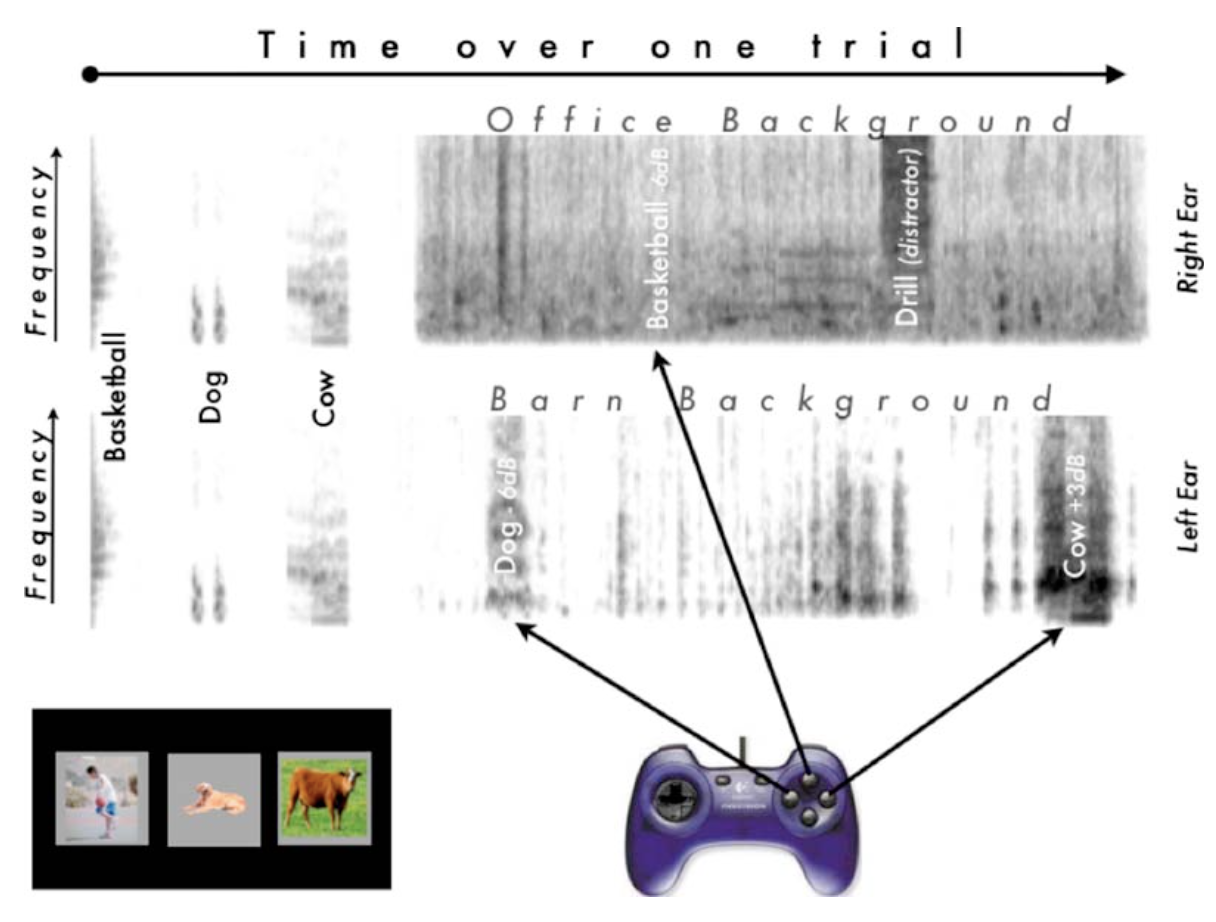
\includegraphics[width=0.65\linewidth]{figures/ENVASAparadigm} 

}

\caption{Schematic of the ENVASA experimental paradigm \autocite[taken from][]{Leech2009}}\label{fig:ENVASA}
\end{figure}

\hypertarget{celf-rs}{%
\subsubsection{CELF-RS}\label{celf-rs}}

The Recalling Sentences (RS) sub-test of the Clinical Evaluation of Language Fundamentals Fifth UK edition \autocite[CELF-5-UK][]{HWiig2017} was administered to assess the listeners expressive language ability and has been shown to be a good indicator of the listeners general language skills (REF). In the task the child is presented with pre-recorded sentences of increasing length and complexity and required to repeat sentences without any changes. Scoring were marked by hand by the examiner as instructed by the test manual. The sentences were spoken by a standard southern British English female and were recorded in a sound-treated recording booth at the SHaPS UCL laboratory, London. The sentences were presented using a MATLAB program via headphones using the same experimental equipment as listed above at a comfortable output level of 70~dB~HL. The task began with two practice sentences while the number of test items varied depending on the child's age performance. No repetitions or feedback was given during the testing and the test was discontinued in case the child failed to score any points for four consecutive items. Age-scaled score were calculated based on the test norms whereby the cut-off scaled score for abnormal performance is \(\leq\)~7. Average scaled score are between 8 to 12 (\(\pm\)~1~SD) while scores \(\geq\)~13 (+1~SD)are classified as above average.

\hypertarget{questionnaires}{%
\subsection{Questionnaires}\label{questionnaires}}

\hypertarget{medical-neurological-and-pysiological-history}{%
\subsubsection*{Medical, Neurological, and Pysiological History}\label{medical-neurological-and-pysiological-history}}
\addcontentsline{toc}{subsubsection}{Medical, Neurological, and Pysiological History}

\hypertarget{the-evaluation-pf-childrens-listening-and-processing-skills-eclips}{%
\subsubsection*{The Evaluation pf Children's Listening and Processing Skills (ECLiPS)}\label{the-evaluation-pf-childrens-listening-and-processing-skills-eclips}}
\addcontentsline{toc}{subsubsection}{The Evaluation pf Children's Listening and Processing Skills (ECLiPS)}

The ECLiPS questionnaire \autocite{Barry2014} comprises of 38 items where the users are asked to express their agreement simple statements about the child's listening and other related skills or behaviours using a five-point Likert scale (from ``strongly agree'' to ``strongly disagree''). The ECLiPS was design to identify listening and communication difficulties in children aged 6 to 11 years. Nonetheless, the UK standardisation study (REF) found little to no age effect on scores in many of the scale items, suggesting the testing age could be extended below and beyond the population used for the development. Based on factor analysis the items are grouped into five subcategories: 1. Speech \& Auditory Processing (SAP), 2. Environmental \& Auditory Sensitivity (EAS), 3. Language, literacy \& laterality (L/L/L), 4. Memory \& Attention (M\&A), 5. Pragmatic \& Social skills (PSS). Age- and sex-scaled scores were computed using the test excel scorer.

A score below the 10\(^{th}\) percentile (corresponding to a scale score of circa 6) is generally considered clinically significant.

\hypertarget{the-childrens-communication-checklist-2nd-edition-ccc-2}{%
\subsubsection*{\texorpdfstring{The Children's Communication Checklist 2\(^{nd}\) edition (CCC-2)}{The Children's Communication Checklist 2\^{}\{nd\} edition (CCC-2)}}\label{the-childrens-communication-checklist-2nd-edition-ccc-2}}
\addcontentsline{toc}{subsubsection}{The Children's Communication Checklist 2\(^{nd}\) edition (CCC-2)}

Communication abilities were assessed using the Children's Communication Checklist second edition questionnaire \autocite[CCC-2;][]{D.V.M.2003} was completed by the child's parent/guardian. The CCC-2 was designed to screen communication problems in children aged 4 to 16 years and comprises of 70 checklist items each comprising of a behaviour statement like ``Mixes up words of similar meaning''. The respondents are asked to judge how often the behaviours occur using a four-point Likert rating scale: 0. \emph{less than once a week (or never)}, 1. \emph{at least once a week, but not every day}, 2. \emph{once or twice a day}, 3. \emph{several times (more than twice) a day (or always)}. The items are grouped into ten sub-scales of behaviours tapping into different skills (A. Speech, B. Syntax, C. Semantics, D. Coherence, E. Inappropriate initiation, F. Stereotyped language, G. Use of context, H. Non-verbal communication, I. Social relations, J. Interests). Taking the sum of scores for the sub-scales A to H are used to derive the General Communication Composite (GCC) which is used to identify clinically abnormal communication competence. A GCC score \textless{} 55 was found by \textcite{Norbury2005} to well separate between control and clinical groups, identifying children with scores at the bottom 10\%. Another composite (Social-Interaction Deviance Composite, SIDC) was taken by taking the difference in sum of scales E, H, I, and J from the sum of scales of A to D. Abnormal GCC (\textless~55) combined with a negative SIDC score has been shown to be indicative of an autistic spectrum disorder profile \autocite{D.V.M.2003}. The CCC-2 scaled and composite scores were computed using the test excel scorer. X observations out of Y were removed from the analysis due to inconsistent reports flagged by the test scorer.

\hypertarget{results-3}{%
\section{Results}\label{results-3}}

\hypertarget{extended-high-frequency-audiometry-ehfa-1}{%
\subsection{Extended high-frequency audiometry (EHFA)}\label{extended-high-frequency-audiometry-ehfa-1}}

The listeners' thresholds for the left and the right ear are plotted in Figure \ref{fig:EHF}. The shaded grey area represents the TD group thresholds range and the white line represents their mean at each frequency. The black lines represents the individual thresholds in the APD group and the group mean is marked by the bold black line.

\colorbox[HTML]{CCCCFF}{Difference in HL between audiogram types?}
First, the quality(?) of the thresholds measured with the non-standard ER10X audiogram was tested by comparing the individuals thresholds with those obtained with the standard audiometer. This was tested group-wise for thresholds at 8~kHz measured in the left and the right ear using Wilcoxon signed rank test for paired samples (rstatix::wilcox\_test with bonferroni adjustment; REF). The test showed a significant difference in thresholds between the two audiogram type for the TD group in both right (p=1, effect size r=0.114) and the left ear (p=1, r=0.092). No significant difference was found in the APD group in both ears (right: p=0.544, r=0.235; left: p=0.844, r=0.2).

\colorbox[HTML]{CCCCFF}{Difference between groups}
Similarly, difference in thresholds between the groups across frequencies (11 \& 16~kHz) and ears (left/right) was tested using a Wilcoxon rank-sum test for unpaired samples (rstatix::wilcox\_test with bonferroni adjustment; REF). No significant difference was found between the groups for all frequency/ear combinations (all p\textgreater.05).

\colorbox[HTML]{CCCCFF}{PTAs and BEs}

The same holds for PTAs (calculated as the mean of thresholds at 11 \& 16~kHz, severalty for the left and the right ear) as well as for PTA at the better ear, where no significant difference was found between the groups. This was tested using a Wilcoxon rank-sum test for unpaired samples with permutation (coin::wilcox\_test, REF).

\begin{figure}

{\centering \includegraphics[width=0.85\linewidth]{_main_files/figure-latex/EHF-1} 

}

\caption{APD participants pure-tone thresholds for extended high-frequencies plotted for the left and the right ear (black). The shaded grey area represents the TD group range of audiometric thresholds and the white line represents the mean at each frequency..}\label{fig:EHF}
\end{figure}

\hypertarget{switching-task-st-1}{%
\subsection{Switching task (ST)}\label{switching-task-st-1}}

\hypertarget{spatialised-speech-in-noise-lisns-uk-1}{%
\subsection{Spatialised speech-in-noise (LiSNS-UK)}\label{spatialised-speech-in-noise-lisns-uk-1}}

\begin{table}

\caption{\label{tab:LiSNS-uRevs}Add caption here...}
\centering
\begin{tabular}[t]{lrrrrrrrrrr}
\toprule
\multicolumn{1}{c}{ } & \multicolumn{5}{c}{TD} & \multicolumn{5}{c}{APD} \\
\cmidrule(l{3pt}r{3pt}){2-6} \cmidrule(l{3pt}r{3pt}){7-11}
condition & n & mean & sd & min & max & n & mean & sd & min & max\\
\midrule
SSN & 23 & -5.31 & 1.42 & -8.05 & -2.00 & 20 & -4.82 & 1.36 & -7.4 & -2.30\\
S0N0 & 23 & -1.79 & 1.90 & -5.55 & 2.95 & 20 & -1.81 & 1.74 & -4.7 & 2.37\\
S0N90 & 23 & -9.07 & 2.55 & -13.50 & -3.42 & 20 & -9.02 & 2.70 & -13.8 & -1.70\\
SRM & 23 & 7.28 & 1.21 & 4.20 & 9.17 & 20 & 7.22 & 2.46 & 1.0 & 11.40\\
\bottomrule
\end{tabular}
\end{table}

Descriptive statistics of the listeners performance split across the two groups is given in Tab. ??. A total of two SRTs were obtained for each participant, one for the spatially collocated (S0N0) and one for the spatially separated (S0N90) listening condition. In addition, the listeners' SRM was calculated by taking the difference between the two conditions (SRM = S0N0 - S0N90).

see Table \ref{tab:LiSNS-uRevs}

\hypertarget{speech-in-noise-spin-1}{%
\subsection{Speech-in-noise (SPIN)}\label{speech-in-noise-spin-1}}

\hypertarget{the-environmental-auditory-scene-analysis-task-envasa-1}{%
\subsection{The Environmental Auditory Scene Analysis task (ENVASA)}\label{the-environmental-auditory-scene-analysis-task-envasa-1}}

\hypertarget{celf-rs-1}{%
\subsection{CELF-RS}\label{celf-rs-1}}

\hypertarget{questionnaires-1}{%
\subsection{Questionnaires}\label{questionnaires-1}}

\hypertarget{discussion-4}{%
\section{Discussion}\label{discussion-4}}

\hypertarget{conclusion-2}{%
\section{Conclusion}\label{conclusion-2}}

\clearpage

\begin{savequote}
Alles Gescheite ist schon gedacht worden.\\
Man muss nur versuchen, es noch einmal zu denken.

All intelligent thoughts have already been thought;\\
what is necessary is only to try to think them again.
\qauthor{--- Johann Wolfgang von Goethe \autocite{von_goethe_wilhelm_1829}}\end{savequote}



\hypertarget{general-discussion}{%
\chapter*{General discussion}\label{general-discussion}}
\addcontentsline{toc}{chapter}{General discussion}

If we don't want Conclusion to have a chapter number next to it, we can add the \texttt{\{-\}} attribute.

\textbf{More info}

And here's some other random info: the first paragraph after a chapter title or section head \emph{shouldn't be} indented, because indents are to tell the reader that you're starting a new paragraph. Since that's obvious after a chapter or section title, proper typesetting doesn't add an indent there.

\hypertarget{summary-of-main-findings}{%
\section*{Summary of main findings}\label{summary-of-main-findings}}
\addcontentsline{toc}{section}{Summary of main findings}

\hypertarget{conclusion-3}{%
\section*{Conclusion}\label{conclusion-3}}
\addcontentsline{toc}{section}{Conclusion}

\startappendices

\hypertarget{the-first-appendix}{%
\chapter{The First Appendix}\label{the-first-appendix}}

This first appendix includes an R chunk that was hidden in the document (using \texttt{echo\ =\ FALSE}) to help with readibility:

\textbf{In 02-rmd-basics-code.Rmd}

\begin{Shaded}
\begin{Highlighting}[]
\KeywordTok{library}\NormalTok{(tidyverse)}
\NormalTok{knitr}\OperatorTok{::}\KeywordTok{include\_graphics}\NormalTok{(}\StringTok{"figures/chunk{-}parts.png"}\NormalTok{)}
\end{Highlighting}
\end{Shaded}

\textbf{And here's another one from the same chapter, i.e.~Chapter \ref{code}:}

\hypertarget{the-second-appendix-for-fun}{%
\chapter{The Second Appendix, for Fun}\label{the-second-appendix-for-fun}}


%%%%% REFERENCES

% JEM: Quote for the top of references (just like a chapter quote if you're using them).  Comment to skip.
% \begin{savequote}[8cm]
% The first kind of intellectual and artistic personality belongs to the hedgehogs, the second to the foxes \dots
%   \qauthor{--- Sir Isaiah Berlin \cite{berlin_hedgehog_2013}}
% \end{savequote}

\setlength{\baselineskip}{0pt} % JEM: Single-space References

{\renewcommand*\MakeUppercase[1]{#1}%
\printbibliography[heading=bibintoc,title={\bibtitle}]}

\end{document}
